\documentclass[12pt, oneside]{article}
\usepackage{geometry}                		% See geometry.pdf to learn the layout options. There are lots.
\geometry{letterpaper} 
\usepackage{amsmath}
\usepackage{amsthm}
\usepackage{amssymb}
\usepackage{graphicx}
\usepackage{color}
\usepackage{float}
\usepackage{subfig}
\usepackage[flushleft]{threeparttable}
\usepackage{gensymb}
\usepackage{multirow}
\usepackage[dvipsnames]{xcolor}
\newcommand{\BibTeX}{\textsc{Bib}\TeX}
%opening
\title{Modifying Files with Rotate Volume}
\author{}

\begin{document}
\maketitle



RotateVolume can be used in order to modify the a flow volume by rotating and flipping it. There are 3 modifications that can be done. 
The first is flipping the volume about a x axis, this will move a wall from bottom to top and vice versa. The other 2 modifications involve rotations and flips in order to
change file dimensions so that the inflow is from the top and the wall is on either the left or right size. None of these modifications should alter anything in the y direction.
Additionally an option was made to output data into plt format for immediate use in tecplot, this was done using code from the tecplot website made by Wen Long. 
Below are figures that show the possible modifications which are chosen using irotate = 2,1 and 3 respectively 


\begin{figure}[H]
\centering
\subfloat[]{\label{fig:} 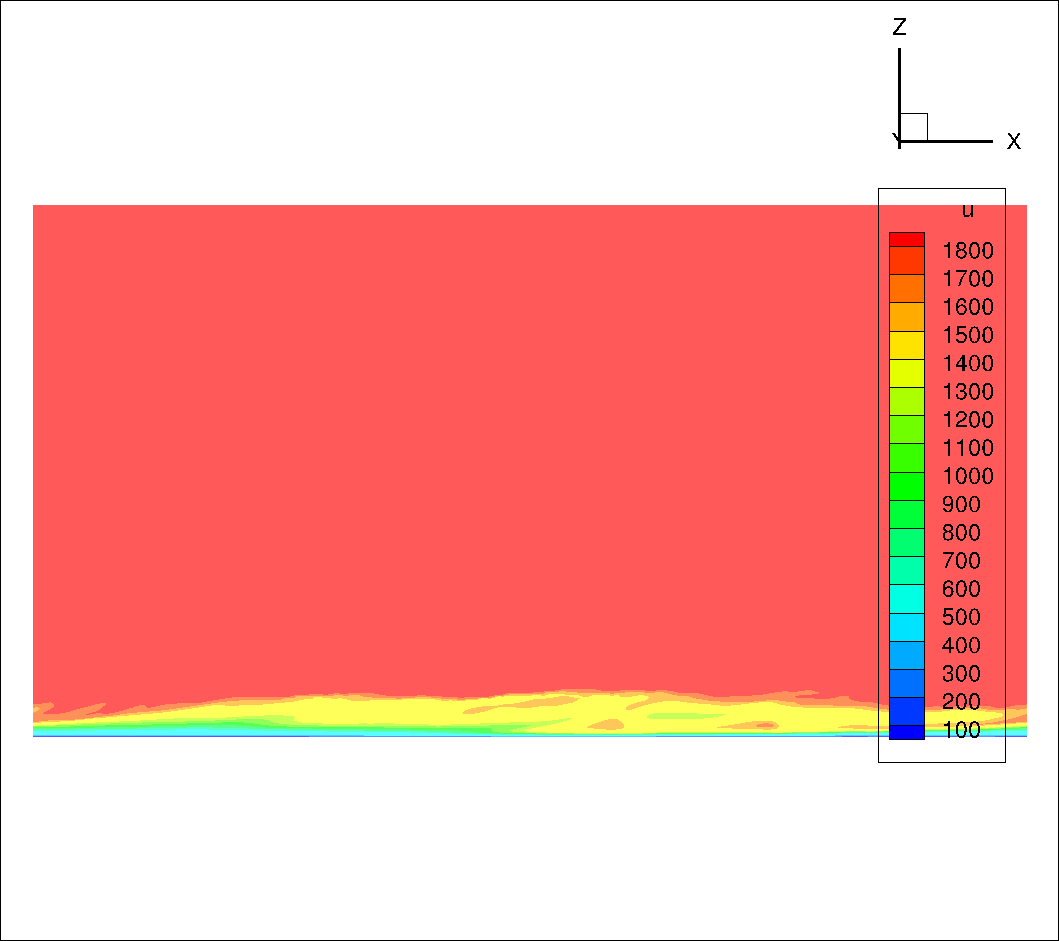
\includegraphics[width=0.5\textwidth]{FIGS/BaseAcous.png}}
\subfloat[]{\label{fig:} 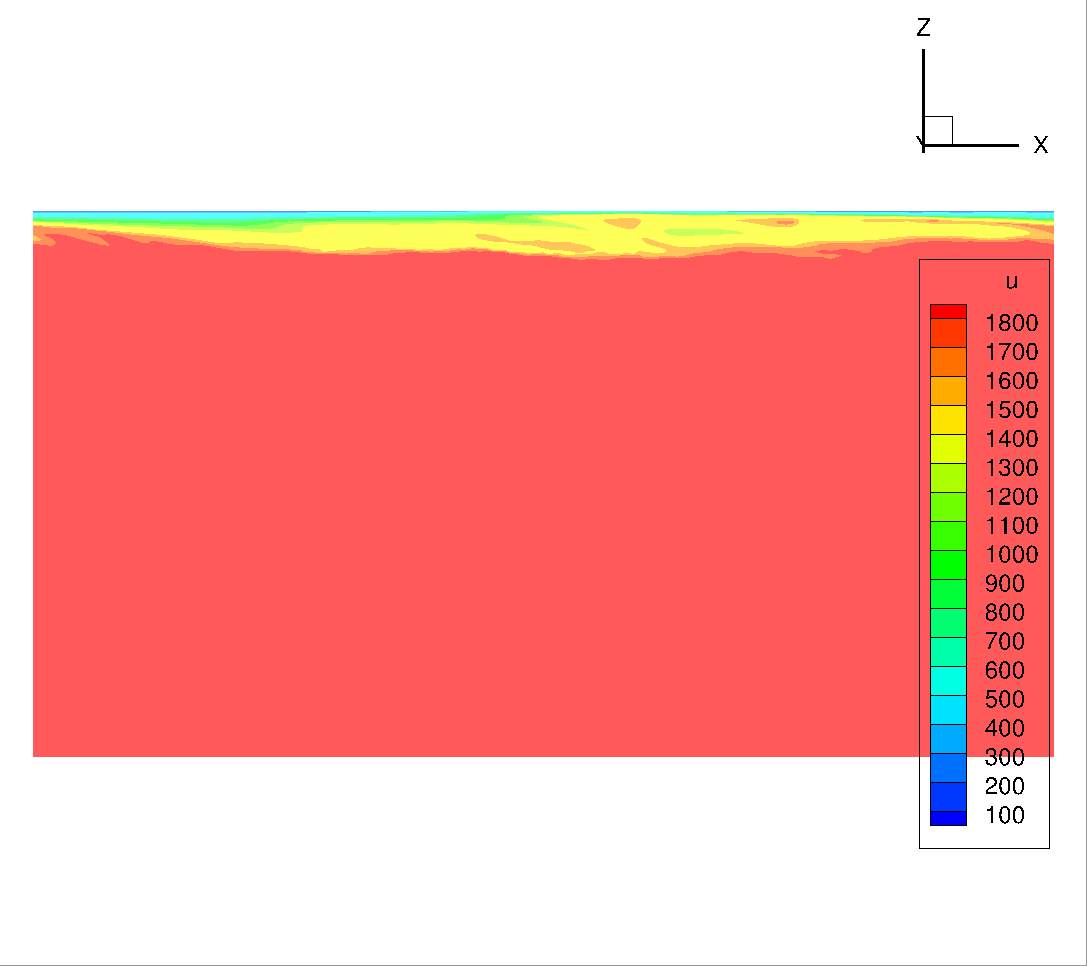
\includegraphics[width=0.5\textwidth]{FIGS/FlipedAcous.png}}

\subfloat[]{\label{fig:} 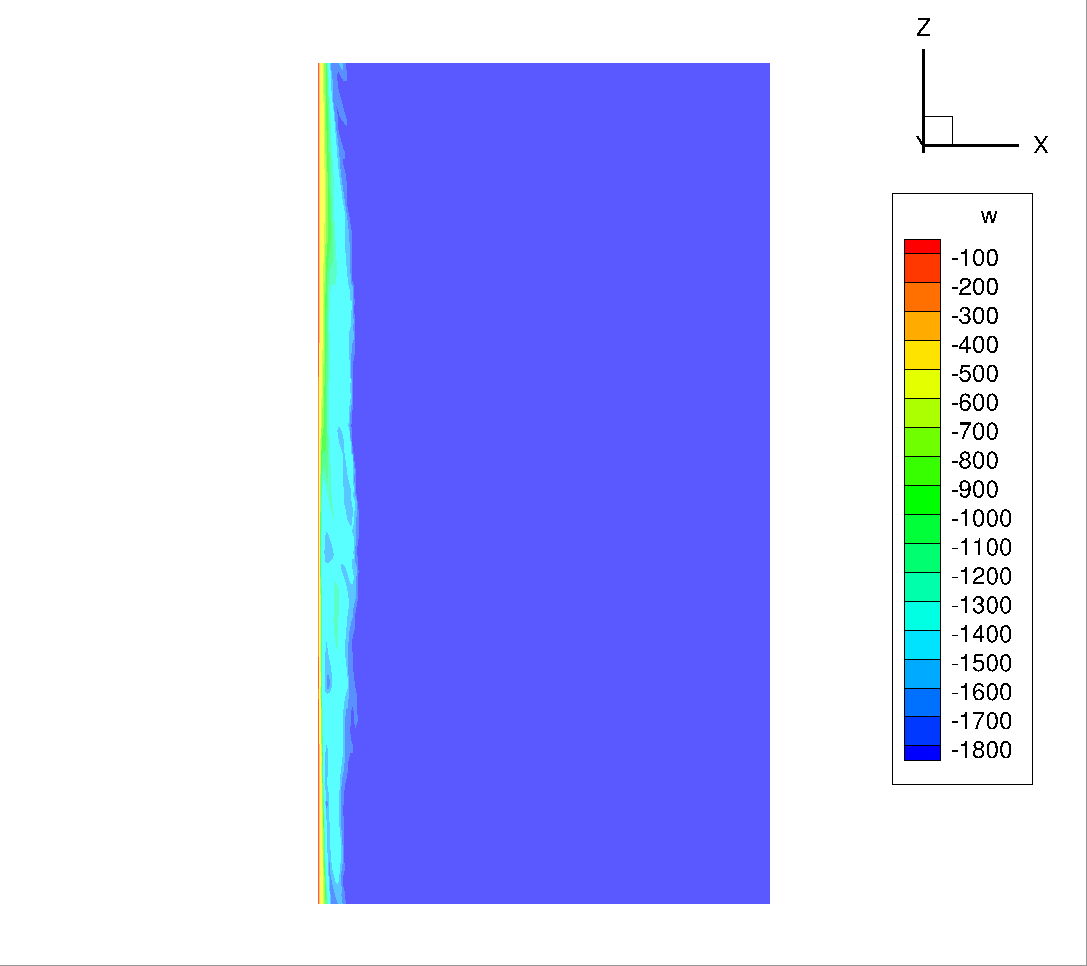
\includegraphics[width=0.5\textwidth]{FIGS/RotCWAcous.png}}
\subfloat[]{\label{fig:} 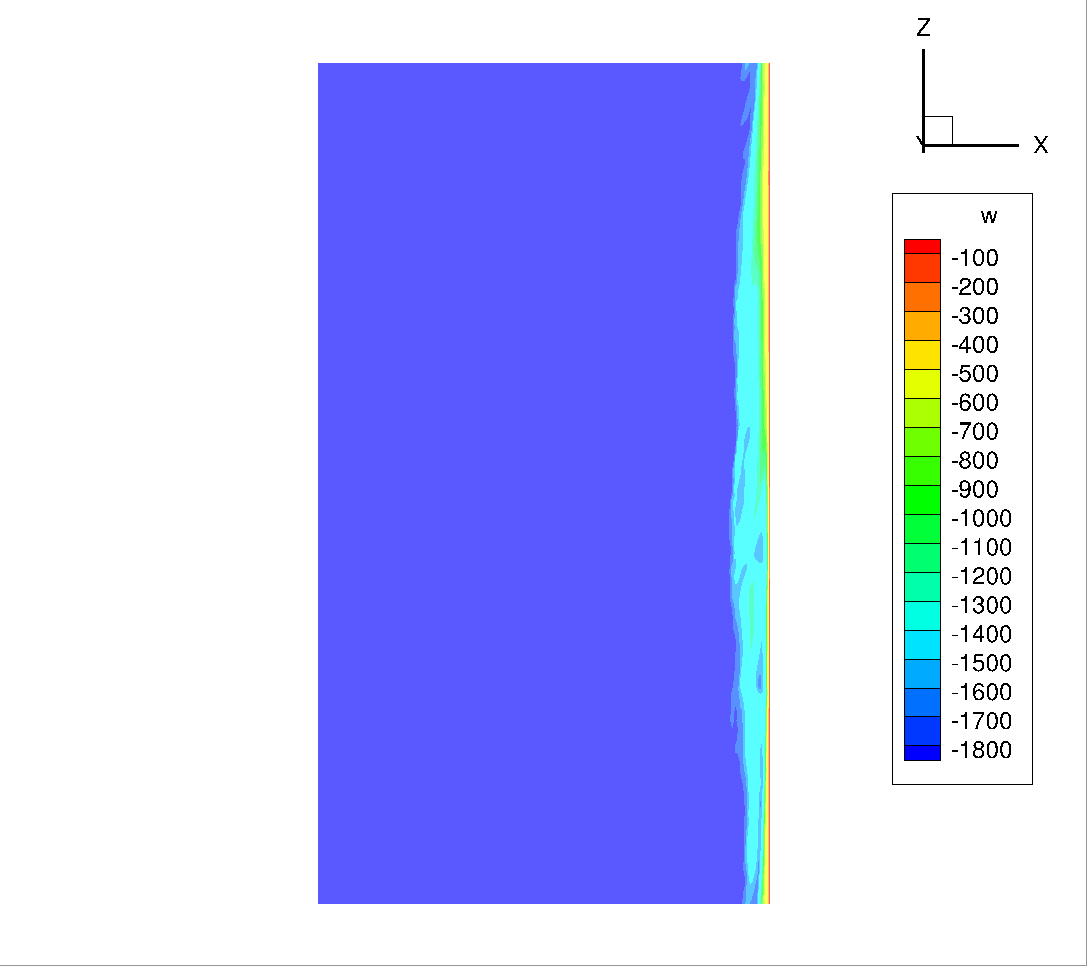
\includegraphics[width=0.5\textwidth]{FIGS/RotCCWAcous.png}}
\caption{{\footnotesize Examples of File Modifications (a)Base Case, (b)Flipping Flow Field, (c) Wall on Left Inlet at Top, (d) Wall on Right Inlet at Top}}
\label{fig: } 
\end{figure}





\begin{figure}[H]
\centering
\subfloat[]{\label{fig:} 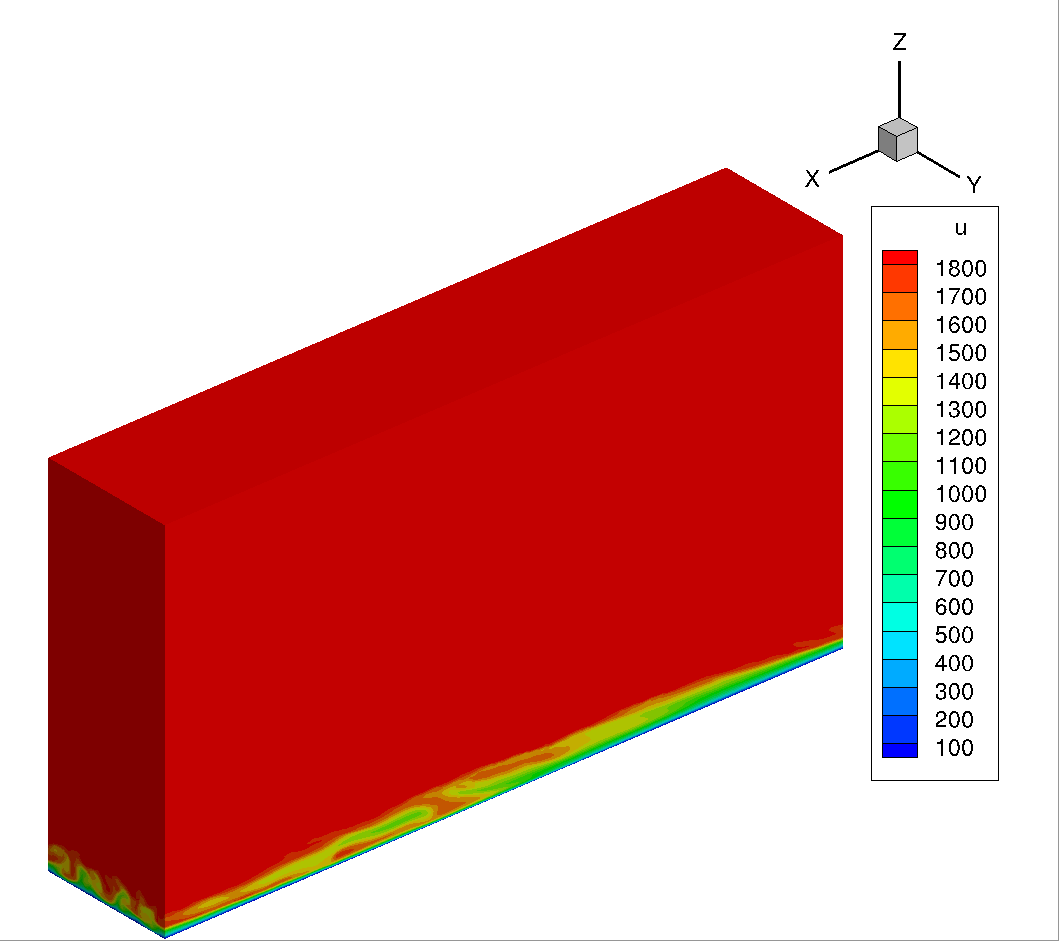
\includegraphics[width=0.5\textwidth]{FIGS/BaseAcous3D.png}}
\subfloat[]{\label{fig:} 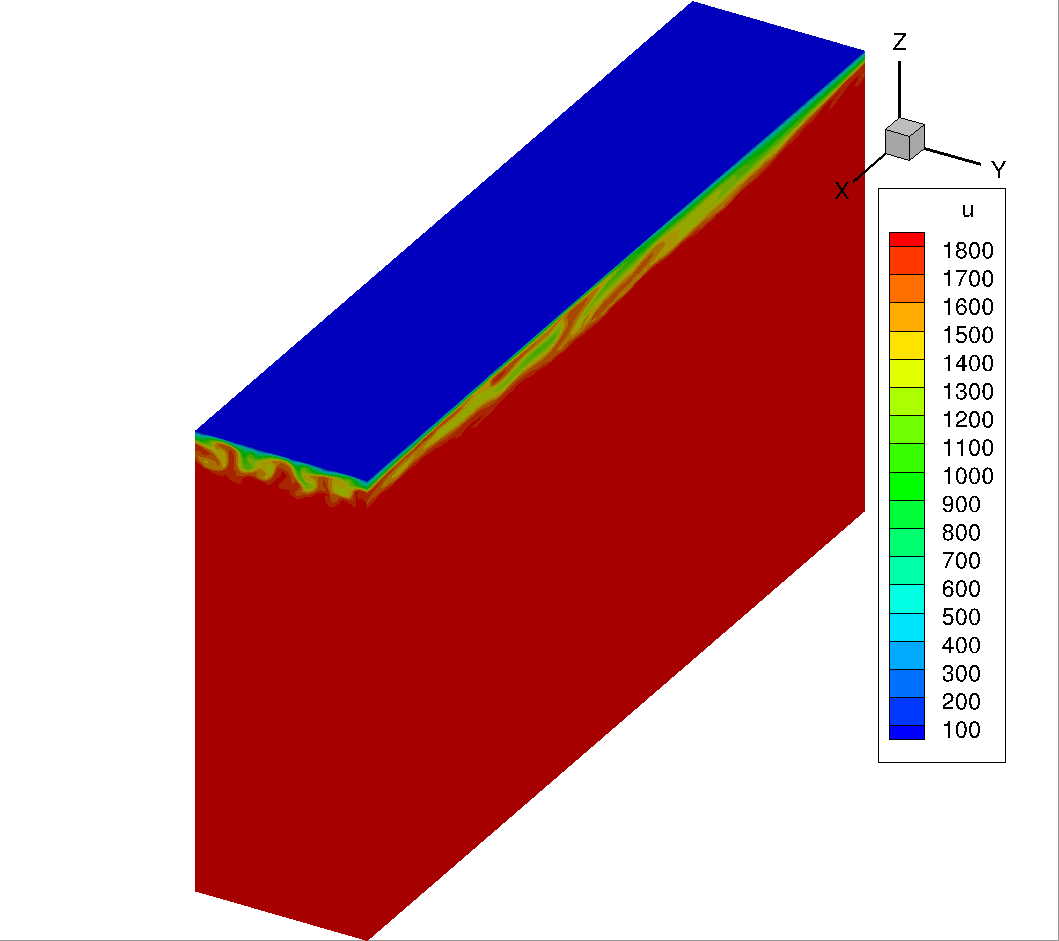
\includegraphics[width=0.5\textwidth]{FIGS/FlipedAcous3D.png}}

\subfloat[]{\label{fig:} 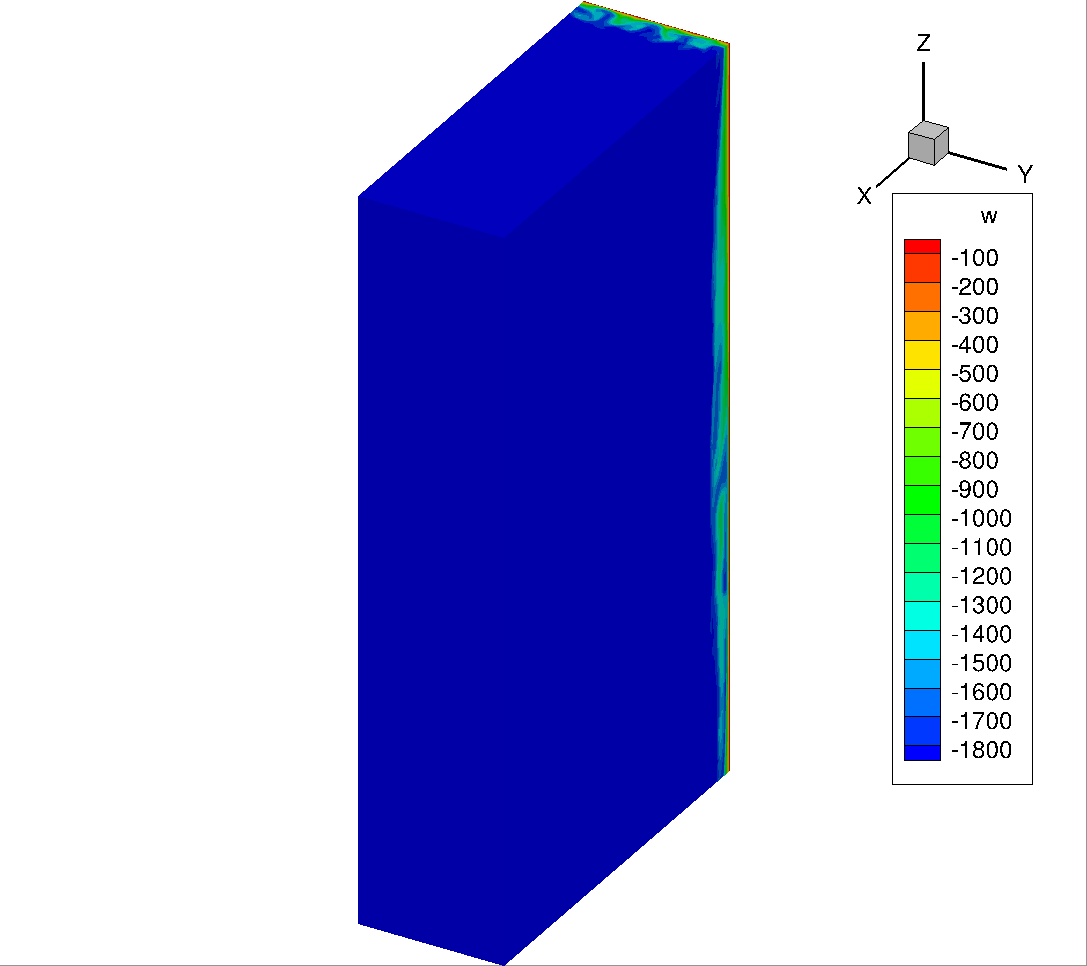
\includegraphics[width=0.5\textwidth]{FIGS/RotCWAcous3D.png}}
\subfloat[]{\label{fig:} 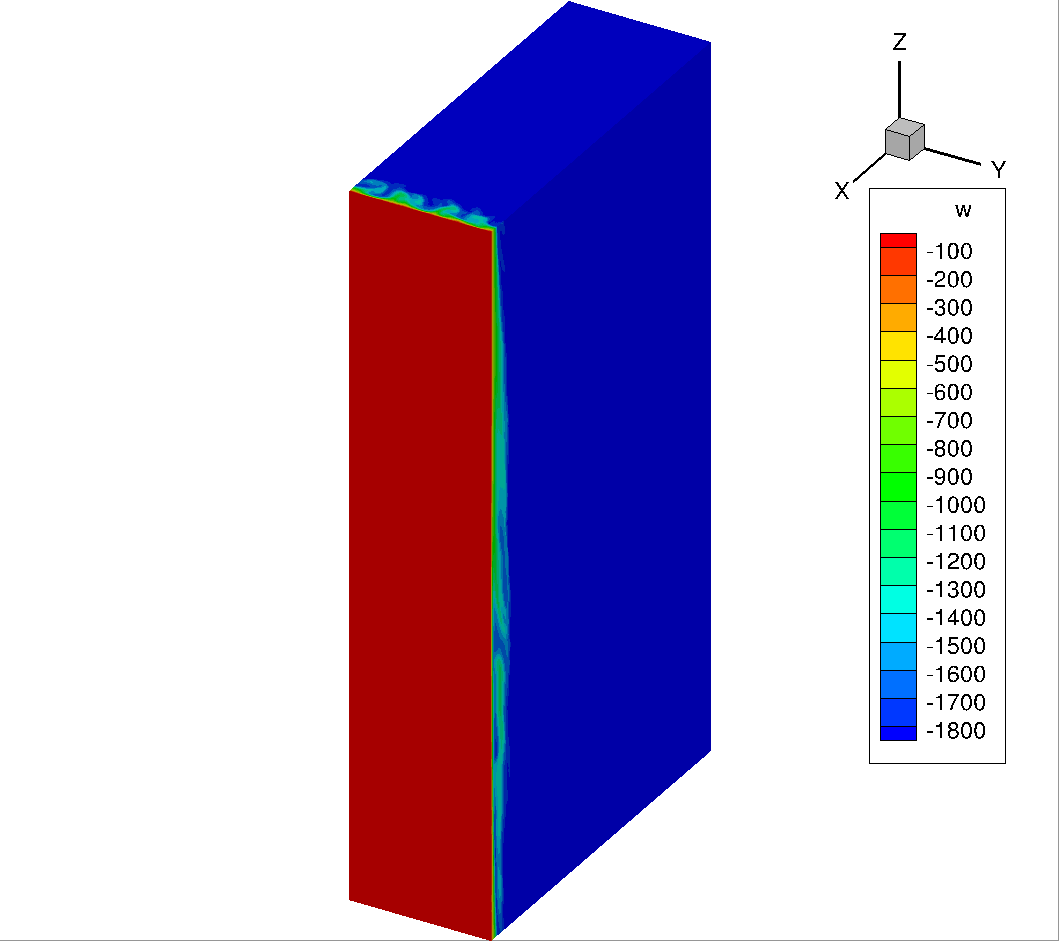
\includegraphics[width=0.5\textwidth]{FIGS/RotCCWAcous3D.png}}
\caption{{\footnotesize Examples of File Modifications 3D View (a)Base Case, (b)Flipping Flow Field, (c) Wall on Left Inlet at Top, (d) Wall on Right Inlet at Top}}
\label{fig: } 
\end{figure}

\begin{figure}[H]
\centering
\subfloat[]{\label{fig:} 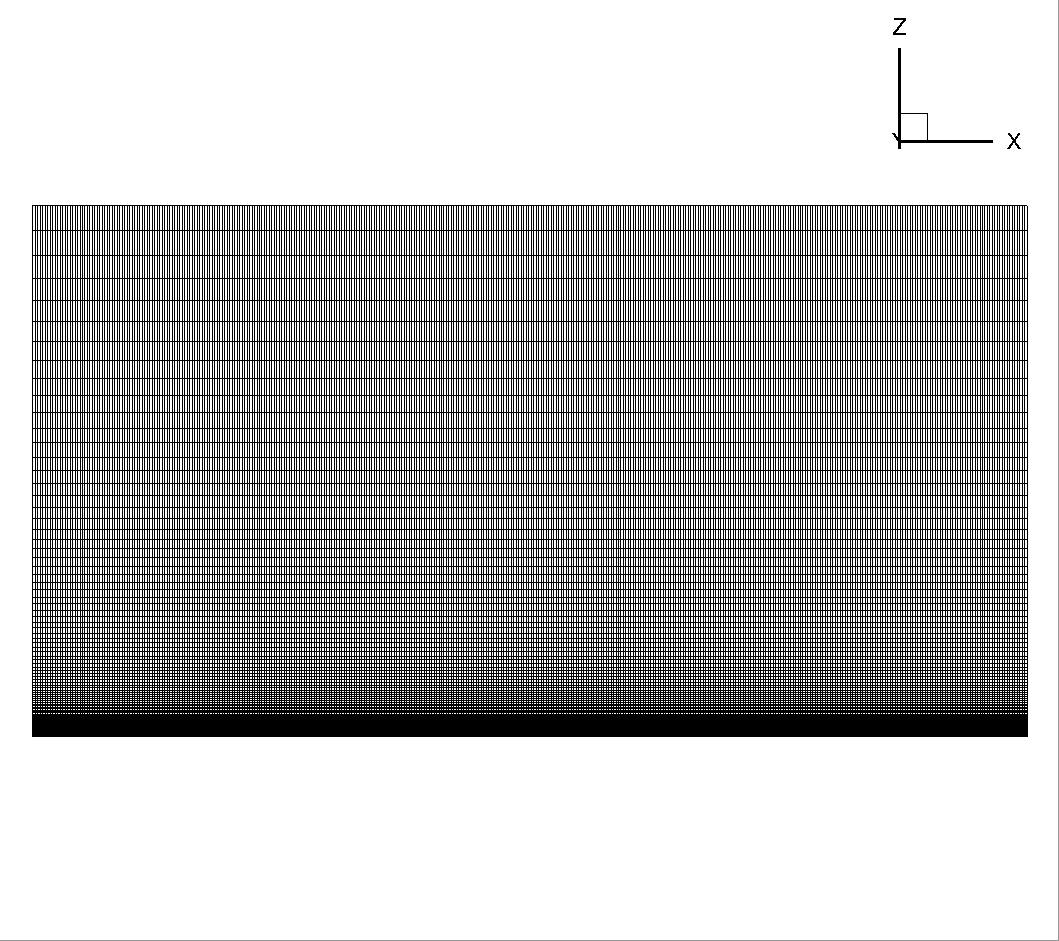
\includegraphics[width=0.5\textwidth]{FIGS/BaseAcousGrid.png}}
\subfloat[]{\label{fig:} 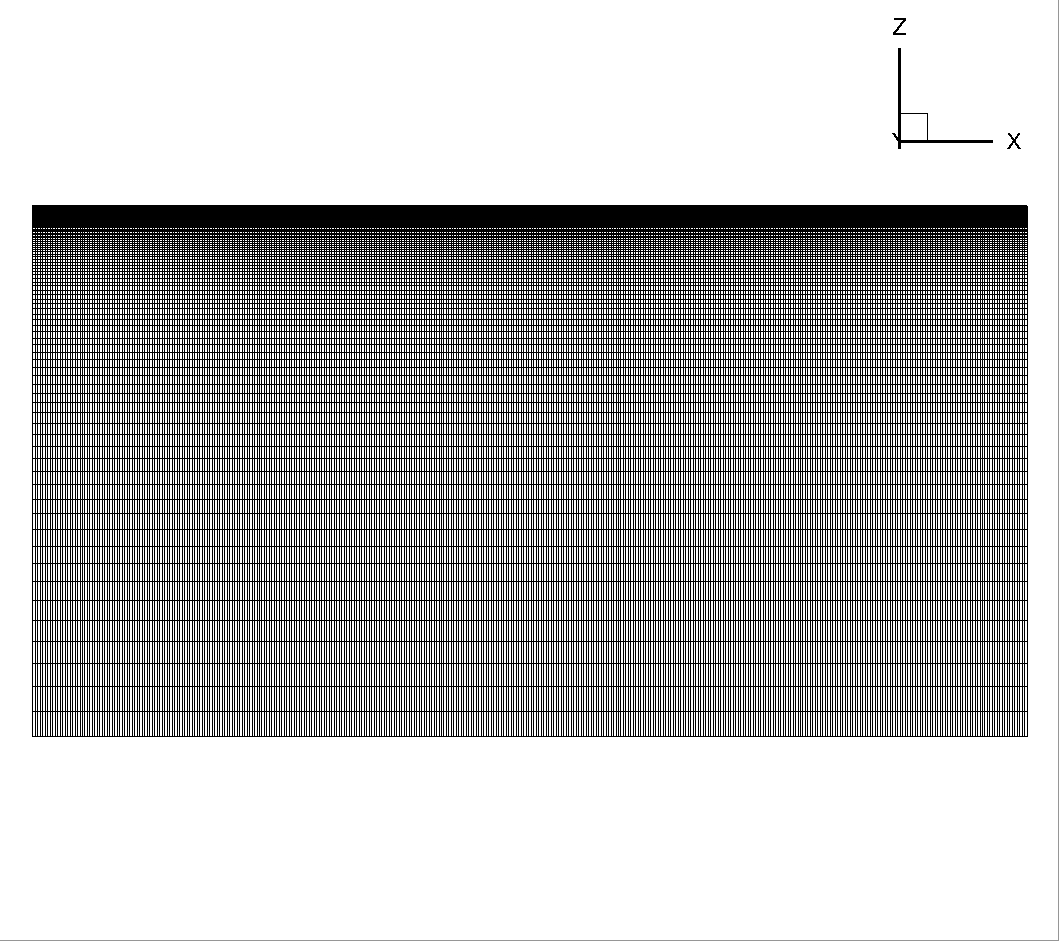
\includegraphics[width=0.5\textwidth]{FIGS/FlipedAcousGrid.png}}

\subfloat[]{\label{fig:} 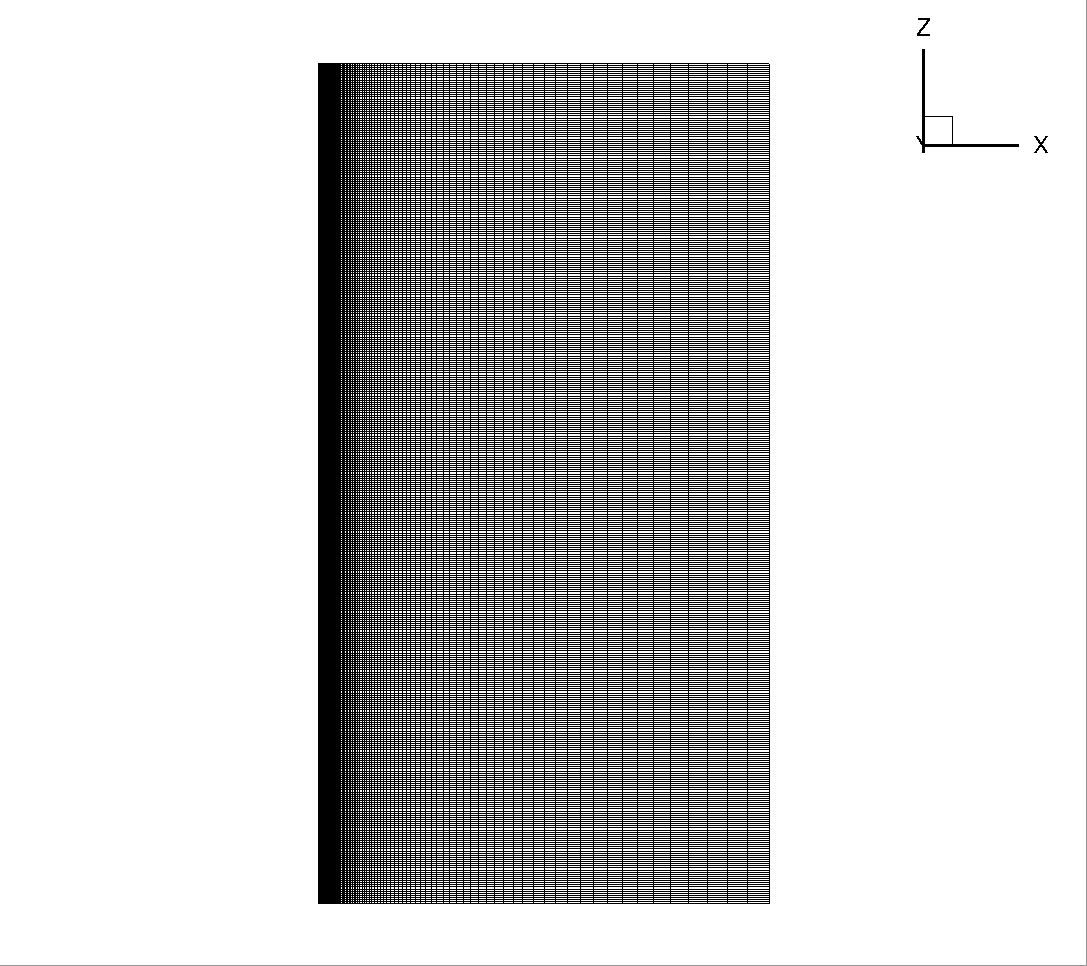
\includegraphics[width=0.5\textwidth]{FIGS/RotCWAcousGrid.png}}
\subfloat[]{\label{fig:} 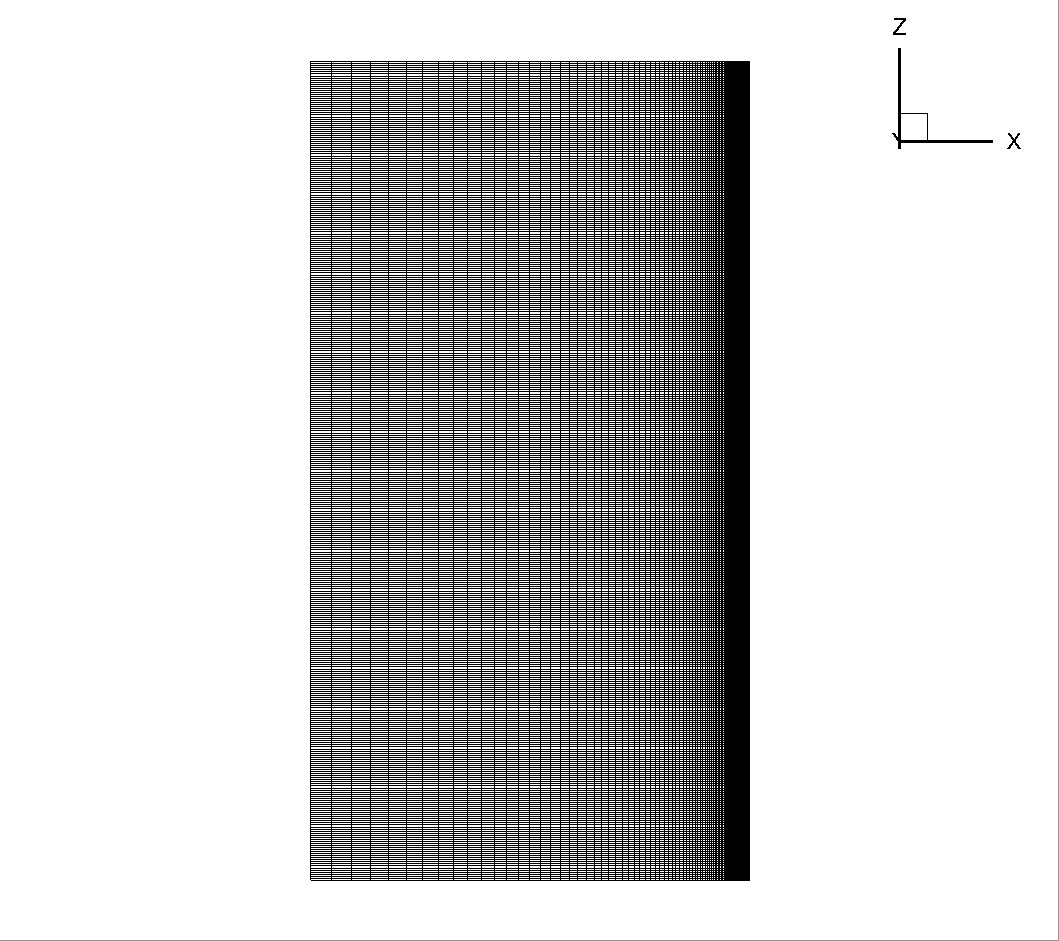
\includegraphics[width=0.5\textwidth]{FIGS/RotCCWAcousGrid.png}}
\caption{{\footnotesize Examples of File Modifications Grids (a)Base Case, (b)Flipping Flow Field, (c) Wall on Left Inlet at Top, (d) Wall on Right Inlet at Top}}
\label{fig: } 
\end{figure}















\end{document}
